\section{A high level overview of Bempp-cl}

\begin{figure}
	\center
	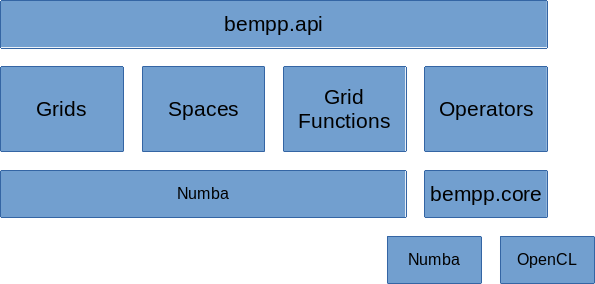
\includegraphics[width=7cm]{img/bempp_overview}
	\caption{The layout of Bempp-cl with its computational backends.}
	\label{fig:overview}
\end{figure}

The main user visible component of Bempp-cl is the module \textbf{bempp.api}, which defines all user interface functions and other high-level routines. In particular, it contains the definition of the main object types: \textbf{Grids}, \textbf{Spaces}, \textbf{Gridfunctions}, \textbf{Operators}. All computational backend routines are part of \textbf{bempp.core}. We are currently supporting a full Numba backend and an OpenCL backend. An overview of this structure is provided in Figure \ref{fig:overview}.

Outside the operator discretisation Numba is used in the following contexts.
\begin{itemize}
	\item Topological computations for the grid. Finding out all neighbour relationships between triangles requires parses through the grid data structure with linear complexity, which is accelerated with Numba.
	\item Definition of local-to-global maps for function spaces. Again, this requires traversal through the grid and assigning relationships between global and local indices.
	\item Grid Functions. A right-hand side function $f$ can be defined as a Python callable. This is just-in-time compiled via Numba and then the product with the corresponding basis functions integrated in each triangle via numerical quadrature, again via Numba accelerated routines.
	\item Sparse matrices. Sparse surface matrices are assembled through Numba accelerated routines.
\end{itemize}

The main computational complexity in discretising the boundary integral equation \eqref{eq:bnd_integral} is coming from the discretisation of the left-hand side integral operator. Using dense methods this has quadratic complexity in the number of surface triangles.

Once the user defines an operator with its associated discretisation spaces and calls the \textbf{weak\_form} method to discretize it the code calls a regular integrator to assemble all the interactions between non-adjacent elements and a singular integrator to compute the interactions between adjacent triangles (only necessary if trial and test space are defined on the same grid). The result is stored internally as a dense Numpy array. The corresponding discretisation routines are proxies that forward to computational routines in either Numba or OpenCL, depending on the user preferences. For OpenCL assembly the code checks additional parameters, such as the default vector length for SIMD operators (e.g. 4 for double precision and 8 for single precision in Intel AVX2, or 1 if a GPU is used), and whether the discretisation should proceed in single or double precision. The OpenCL kernel is then compiled for the underlying compute device using PyOpenCL and executed. If the computational backend is Numba, the call is forwarded to the corresponding Numba discretisation routines and executed. For simple piecewise constant function spaces or other spaces, where the support of each basis function is localized to a single triangle, only one call to the computational routines is necessary. If the support of basis functions is larger than a single triangle different threads may need to sum into the same global degree of freedom. We discuss this in more detail in Section \ref{sec:coloring}.

